The set of data points we are given in this problem can be described by the following linear data fitting model:


\begin{equation}
y_i = \alpha t_i + \beta + e_i  
\label{1}
\end{equation}
\[
e_i \sim N(0,\sigma^2)
\]

Where $e_i$ corresponds to the residual associated with the data point $i$. We shall write equation \ref{1} in matrix  form:

\begin{equation}
\mathbf{b} = \mathbf{A} \mathbf{x} + \mathbf{r}  
\end{equation}
 
And

\[
\mathbf{A} = \begin{bmatrix}
\mathbf{1} & \mathbf{t}
\end{bmatrix}
\qquad
\mathbf{x}= \begin{bmatrix}
\mathbf{\alpha} \\
\mathbf{\beta}
\end{bmatrix}
\quad \mathbf{b} = \mathbf{y}
\]

Where $\mathbf{t}$ and $\mathbf{b}$ are vectors containing the coordinates of the data points, $\mathbf{r}$ is the vector of residuals, and $\mathbf{1}$ is a vector of ones which is the same length as $\mathbf{t}$.	

We are going to study four different ways of estimating the parameters $\alpha$ and $\beta$ of our approximating model, and analyze their performance in the presence of outliers. When applicable, the objective function will be reformulated in a way that allows us to solve the function using \matlab optimization functions linprog and quadprog (code snippets can be found in Appendix \ref{code:part1}). 

Finally, statistical analyses are provided throughout to compare the different methods and their respective advantages/ disadvantages. Mathematical formulas implemented for our statistical results are included in Appendix \ref{stats:formulas}.

\subsection{Introduction}

Figure \ref{fig:dataPlot} shows the measured data (from Problem1Data.mat) along with the true model. Three data points deviate substantially from the rest of the data and will be regarded as outliers. These outliers could result from errors in the measuring device that records the data, or could be considered data points coming from a different statistical distribution. In this specific data set, the outlier case is obvious. However, there are many instances where classifying outliers is less clear-cut decision and therefore more uncertain from the modeller's perspective. Because of this, ideally we would want an approximating model that can incorporate outlier data without negatively affecting its performance. This would lead to a robust estimator or, said differently, a robust regressor. With this goal in mind, the outliers in the plot below will be included in our models. To avoid statistical biases however, the outliers will be discarded during our statistical tests (e.g. confidence intervals, std. deviation of the noise, etc). 

\vspace*{\fill} 
\begin{figure}[htb]
\centering
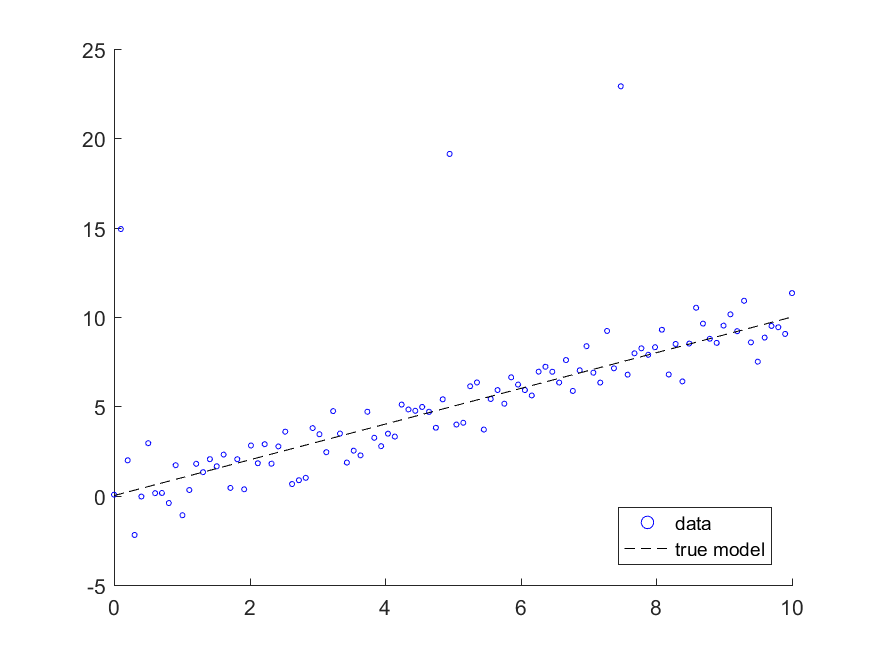
\includegraphics[width=0.6\textwidth]{../img/data_plot}
\caption{Scatter plot of the data}
\label{fig:dataPlot}
\end{figure}
\vspace*{\fill} 

\subsection{Least Squares Estimation}

The least squares estimation is by far the most common method used for determining the parameters of a data fitting model. The objective function is solved, as the name implies, by finding the parameters that minimize the sum of the squared residuals. The $\frac{1}{2}$ is introduced for mathematical computational ease and does not affect the parameter estimates.

\begin{equation}
\min\limits_{x \in \mathbb{R}^n} F(x) = \frac{1}{2} \Vert{\mathbf{A x - b}}\Vert^2_2
\label{eq:leastSquares}
\end{equation}

\vspace*{\fill} 
\newpage
Equation \ref{eq:leastSquares} can be rewritten as:

\begin{equation}
\begin{split}
F(x) &= \frac{1}{2} \Vert\mathbf{{A x - b}}\Vert^2_2 = \frac{1}{2} \mathbf{(A x - b)}'\mathbf{(A x - b)} \\
&=  \frac{1}{2} \mathbf{x' A' A x} + \mathbf{(-A' b)'x} + \frac{1}{2} \mathbf{b' b} \\
&= \frac{1}{2} \mathbf{x' H x} + \mathbf{g' x} + \gamma
\end{split}
\label{eq:leastSquares2}
\end{equation}

Where:

\[
\mathbf{H} = \mathbf{A' A} \qquad \mathbf{g} = \mathbf{-A' b} \qquad \gamma = \frac{1}{2} \mathbf{b' b}
\]

The minimum of the quadratic problem in equation \ref{eq:leastSquares2} can be obtained in \matlab using the optimization function quadprog.

Figure \ref{fig:leastSquares} shows the model obtained with the least squares method. Note that the outliers are incorporated in the model. The L2 model closely resembles the true model except for a minor offset in the y-intercept ($\beta$ estimate). The reader is referred to table 1 in section 1.6 for further detailed results and discussion.  

\begin{figure}[htb]
\centering
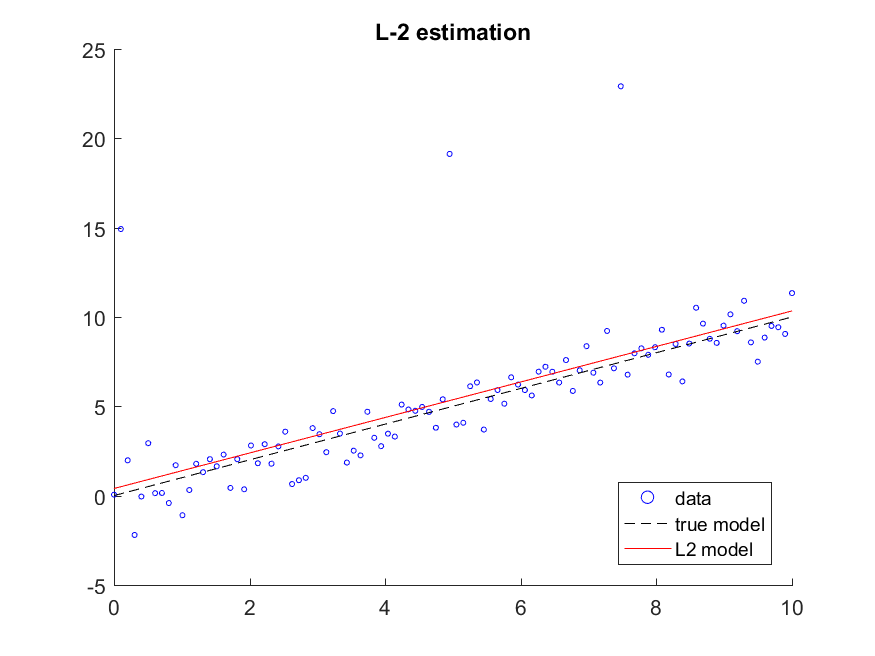
\includegraphics[width=0.6\textwidth]{../img/L2_norm}
\caption{$L_2$ estimation}
\label{fig:leastSquares}
\end{figure}	

The upper-half of Figure \ref{fig:leastSquaresHist} shows a histogram of the residuals when including the outliers; in the bottom-half histogram, the outliers have been removed resulting in the familiar shape of the gaussian distribution. As such, we consider the residuals to be "white noise." The standard deviation of the noise in the L2 model is 1.1228 compared to 1.0293, which is the true noise of the data (see Table 1).    

\begin{figure}[htb]
\centering
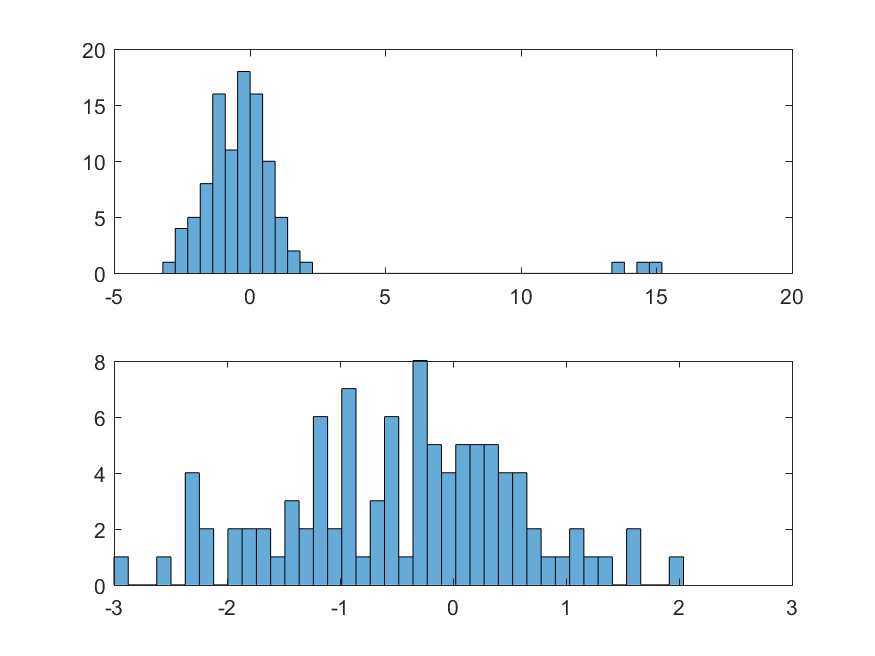
\includegraphics[width=0.6\textwidth]{../img/L2_hist}
\caption{$L_2$ histogram of the errors}
\label{fig:leastSquaresHist}
\end{figure}


The $95\%$ confidence interval of both the parameters and the predictions of the L2 model are shown in Figure \ref{fig:leastSquaresCI}. Notice that the L2 model overestimates the data. That is, most of the data points lie beneath the model. This is due to the L2 model overestimating the $\beta$ parameter presumably due to the upward influence of the three large positive outliers. The small offset in the estimated $\beta$ can be seen in the figure's y-axis - recall that the true $\beta$ equals 0. 
 
The room between the two green lines in figure \ref{fig:leastSquaresCI} represents the confidence interval, and it is the space where $95 \%$ of the time the expected value of a prediction will lie. This should not be confused with another type of interval called prediction interval, which outlines the bounds where a single new observation will lie $95\%$ of the time. The latter accounts for both, the uncertainty of the mean value and the variability of the data. An example of a prediction interval can be seen in figure \ref{fig:L2PI} in Appendix \ref{pred:interval}. 

On the other hand, the brown dashed lines represent the amount of variation one could expect from the parameters if the model was estimated from a different sample population. In other words, since the estimates would not be identical depending on the sample pool they were estimated from, the parameter confidence intervals tell us how much the estimates could vary from sample to sample.  That is, if the experiment was to be carried out 100 times, we would expect the parameters to lie within these intervals $95 \%$ of the time. The numerical values of the parameter estimates and their confidence intervals for each model are listed in Table 3. 

\begin{figure}[htb]
\centering
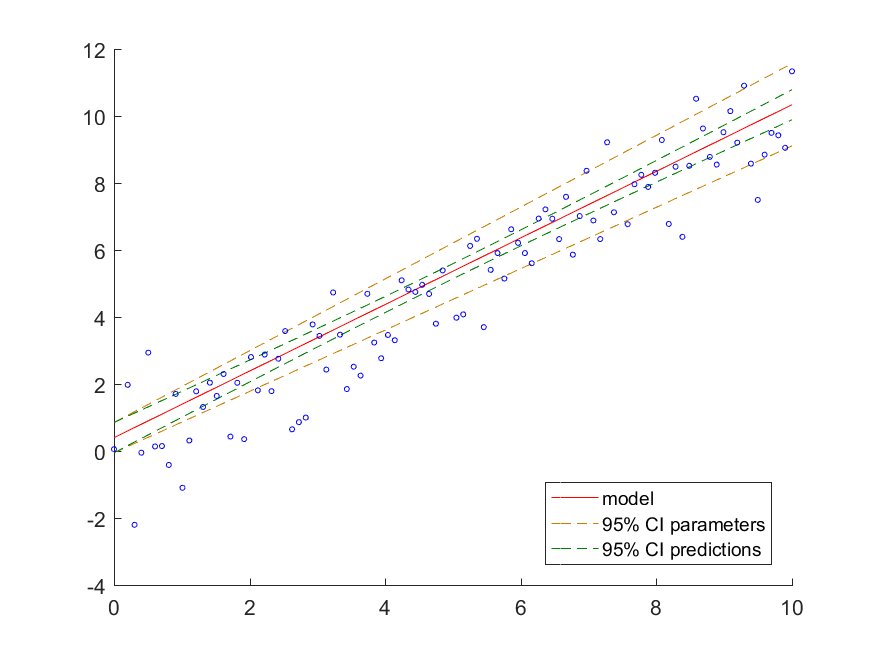
\includegraphics[width=0.6\textwidth]{../img/L2_CI}
\caption{$L_2$ confidence intervals}
\label{fig:leastSquaresCI}
\end{figure}

\newpage 
\subsection{$L_1$ Estimation}

The $L_1$ regression is now obtained by minimizing the sum of the residuals' absolute value. The absolute value function, however, is not smooth. That is, the function is not differentiable at every point, thus the problem must be reformulated. 

A technique that circumvents this problem involves defining a smooth function that envelopes the kinks of the absolute value function. These functions are merged resulting in a kinkless absolute value function. 

\begin{equation}
\min\limits_{x \in \mathbb{R}^n} F(x) =  \Vert A x - b \Vert_1 =  \sum_{i=1}^{m} \vert A x - b \vert
\label{eq:l1estimation}
\end{equation}

The above equation can be expressed as:


\begin{equation}
\min\limits_{x \in \mathbb{R}^n} F(x) =\sum_{i=1}^{m} t_i
\label{eq:l1estimation2}
\end{equation}

\[
t_i \geq \vert{r_i(x)}\vert \qquad i = 1,2,...,m
\]


As can be seen, the problem becomes a linear constrained optimization problem which can be solved using \matlab optimization tool linprog. Before calling the function we must write the problem in matrix form and thus, equation \ref{eq:l1estimation2} becomes:

\begin{equation}
F(x,t) =  \sum_{i=1}^{m} t_i = \begin{bmatrix}
\mathbf{0} \\
\mathbf{1}
\end{bmatrix}' 
\begin{bmatrix}
\mathbf{x} \\
\mathbf{t}
\end{bmatrix}
\label{eq:l1estimation3}
\end{equation}

Where $\mathbf{0}$ is a vector of zeros which is the same length as $\mathbf{x}$, and $\mathbf{1}$ is again a vector of ones of length $m$ equal to the number of data points. The vector $\mathbf{t}$ contains $m$ new parameters.

\[
\mathbf{t} \geq \vert \mathbf{A} \mathbf{x} - \mathbf{b} \vert \leftrightarrow -\mathbf{t} \leq \mathbf{A x} - \mathbf{b} \leq \mathbf{t}
\]

\begin{figure}[H]
\centering
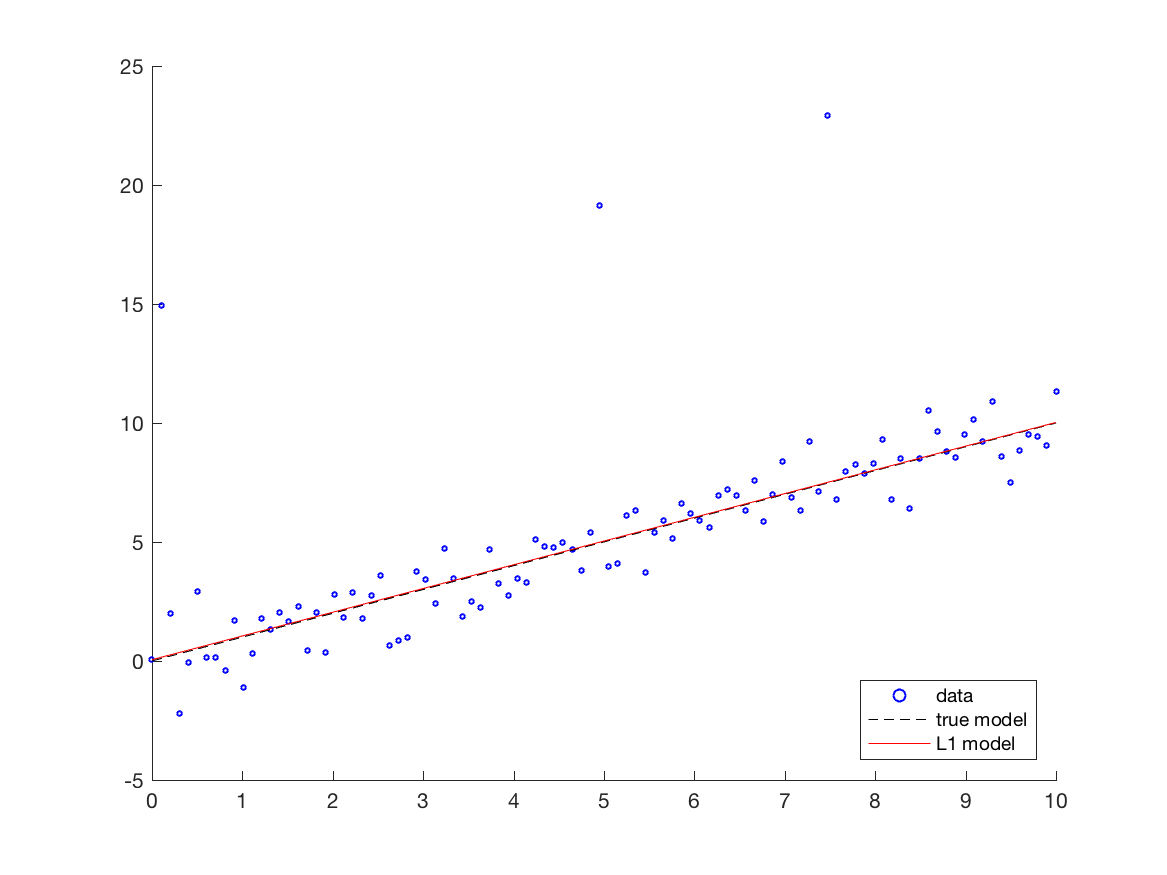
\includegraphics[width=0.6\textwidth]{../img/L1_norm}
\caption{$L_1$ estimation}
\label{fig:l1estimation}
\end{figure}

\begin{figure}[htb]
\centering
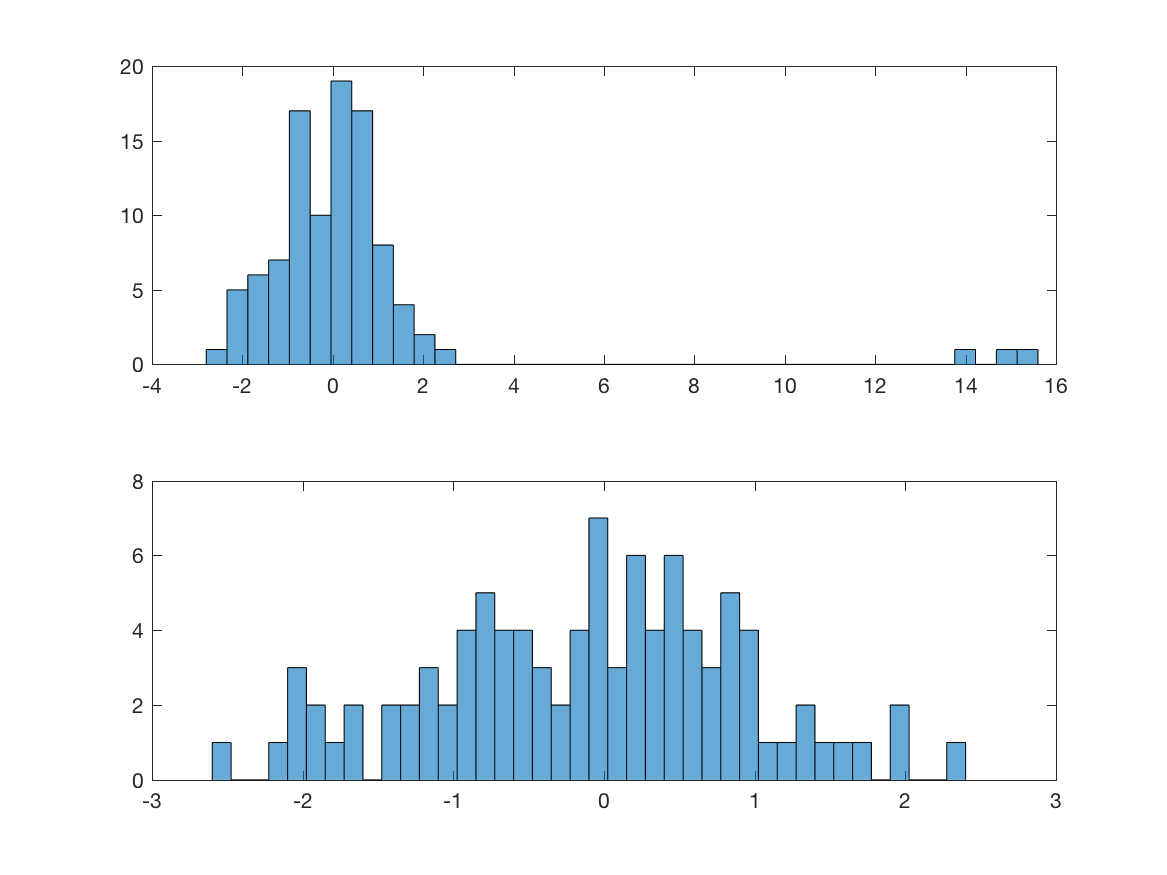
\includegraphics[width=0.6\textwidth]{../img/L1_hist}
\caption{$L_1$ histogram of the residuals}
\label{fig:l1Hist}
\end{figure}	

We reformulate in matrix notation as:

\[
\begin{bmatrix}
\mathbf{A} & \mathbf{I} \\
\mathbf{-A} & \mathbf{I} \\

\end{bmatrix} 
\begin{bmatrix}
\mathbf{x}\\
\mathbf{t}
\end{bmatrix}
\geq 
\begin{bmatrix}
\mathbf{b}\\
-\mathbf{b}
\end{bmatrix}
\]

where $\mathbf{I}$ is the $m \times m$ identity matrix. Note that given how the problem is formulated, the linprog function finds estimates for both $\mathbf{x}$ and  $\mathbf{t}$ vectors even though we are only interested in $\mathbf{x} = \begin{bmatrix} \alpha & \beta \end{bmatrix}'$. We discard $\textbf{t}$ in our analyses. 

Notice that the linprog function requires the inequality to have opposite signs from how we have formulated above. We can simply change the signs to both sides of the inequality and pass the arguments to the function. 

\begin{figure}[htb]
\centering
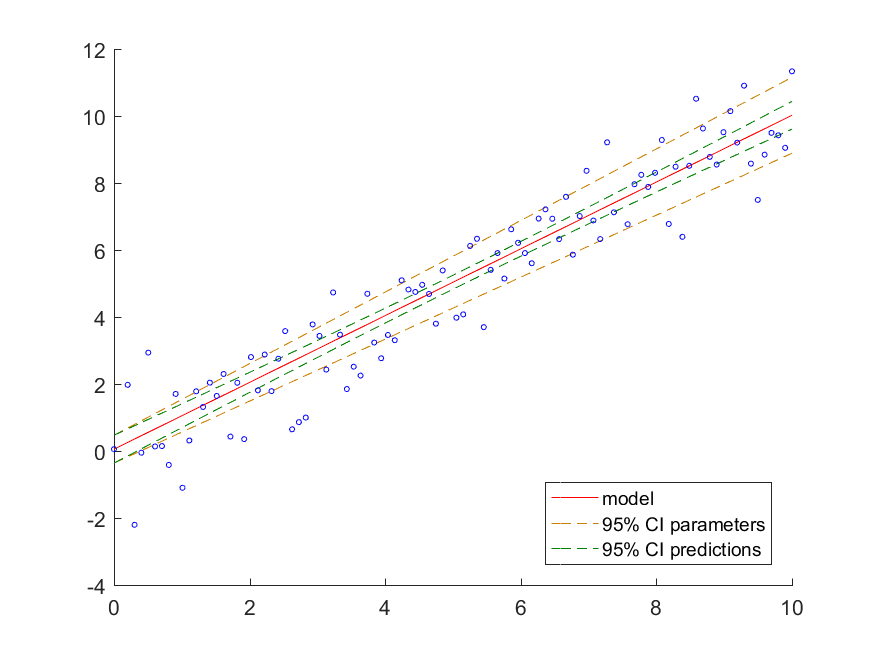
\includegraphics[width=0.6\textwidth]{../img/L1_CI}
\caption{$L_1$ confidence intervals}
\label{fig:l1CI}
\end{figure}

Figure \ref{fig:l1estimation} shows how the L1 model performs relative to the true model. It matches it very closely and we can conclude that the L1-estimation is very robust, at least in our data sample, even in the presence of outliers.

Since the estimated parameters are approximately equal to the true parameters, the residual vector is almost identical to the pure data noise. That is why the histogram in figure \ref{fig:l1Hist} looks like a normal distribution and thus, the residuals, as in the $L_2$ case, can be considered white noise.The certainty of the predictions and the estimated parameters is shown in figure \ref{fig:l1CI}.

\subsection{$L_\infty$ Estimation}

The $L_\infty$ model minimizes the largest of the residuals. 

\begin{equation}
\min\limits_{x \in \mathbb{R}^n} F(x) =  \Vert A x - b \Vert_\infty =  \max\limits_{i \in {1,2,...,m}} \vert A x - b \vert
\label{eq:lInfestimation}
\end{equation}

As in the $L_1$ case, the function is not smooth so we must modify equation \ref{eq:lInfestimation} in order to compute a solution. To do this,we include a new parameter $t$ and set bounds to our problem.

\begin{equation}
\min\limits_{x \in \mathbb{R}^n} F(x,t) = t
\label{eq:lInfestimation2}
\end{equation}
\[
t \geq \vert{r_i(x)}\vert \qquad i = 1,2,...,m
\]

We end up with a constrained linear system that can be expressed in matrix form as:

\begin{equation}
F(x,t) =  \sum_{i=1}^{m} t_i = \begin{bmatrix}
\mathbf{0} \\
1
\end{bmatrix}' 
\begin{bmatrix}
\mathbf{x} \\
t
\end{bmatrix}
\label{eq:lInfestimation3}
\end{equation}

where $\mathbf{0}$ is again a vector of zeros of length equal to the number of data points; the number 1 in the matrix is just a single value.

\begin{figure}[htb]
\centering
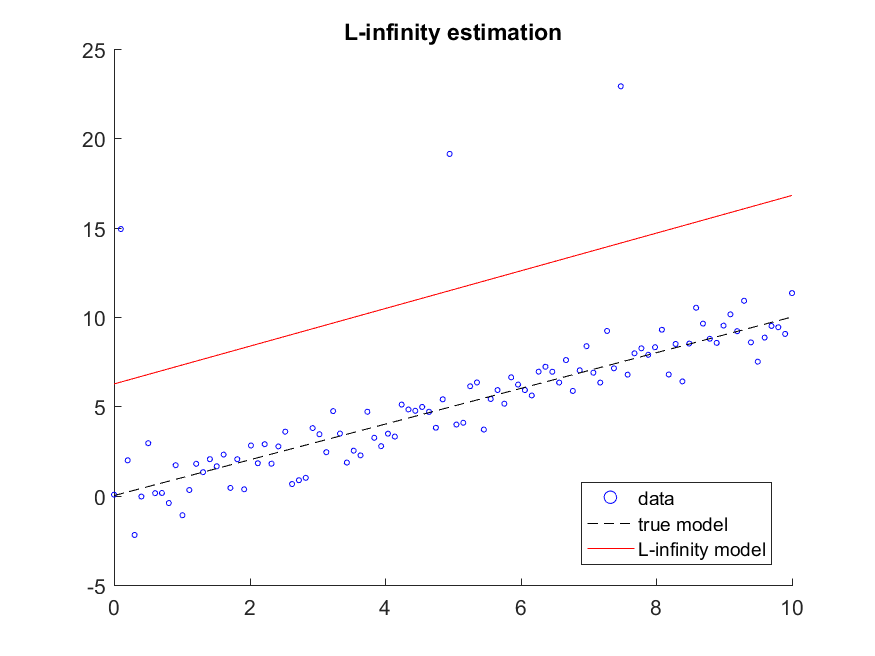
\includegraphics[width=0.6\textwidth]{../img/LInf_norm}
\caption{$L_\infty$ estimation}
\label{fig:lInfestimation}
\end{figure}

From equation number \ref{eq:lInfestimation2} we see that the constant $t$ must be larger than the largest of the residuals, and therefore we shall formulated as:

\[
t [\mathbf{1}] \geq \vert \mathbf{A x} - \mathbf{b}\vert \leftrightarrow -t [\mathbf{1}]  \leq \mathbf{A x} - \mathbf{b} \leq t [\mathbf{1}]
\]

With $\mathbf{1}$ being a length $m$ vector of ones.

\[
\begin{bmatrix}
\mathbf{A} & \mathbf{1} \\
\mathbf{-A} & \mathbf{1} \\
\end{bmatrix} 
\begin{bmatrix}
\mathbf{x}\\
t
\end{bmatrix}
\geq 
\begin{bmatrix}
\mathbf{b}\\
-\mathbf{b}
\end{bmatrix}
\]

As in $L_1$, if we want to use linprog we must change the sign of the inequality. The function will then yield a vector containing the parameters of our model plus the constant $t$. The red line in figure \ref{fig:lInfestimation} represents our estimated model which in this case seems to be very much affected by the outliers.

Using the formulas in Appendix we computed the statistical values for the noise and the estimated parameters. We see in table 3 that the values are now significantly distant to those of the true model. We shall then conclude that the $L_\infty$ model is not a good estimator as it fails to capture the behavior of the data.

\begin{figure}[htb]
\centering
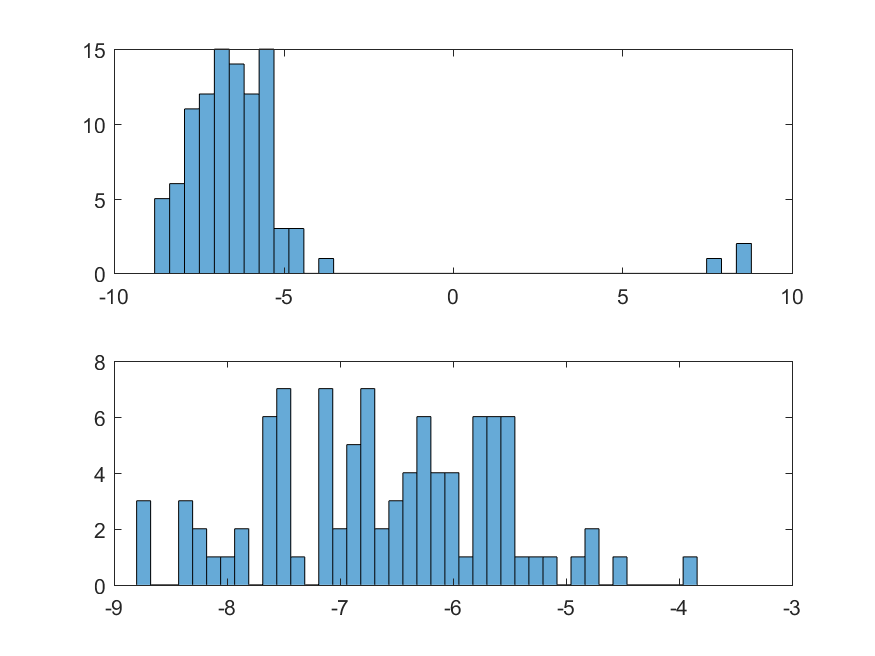
\includegraphics[width=0.6\textwidth]{../img/LInf_hist}
\caption{$L_\infty$ histogram of the errors}
\label{fig:lInfHist}
\end{figure}

\begin{figure}[htb]
\centering
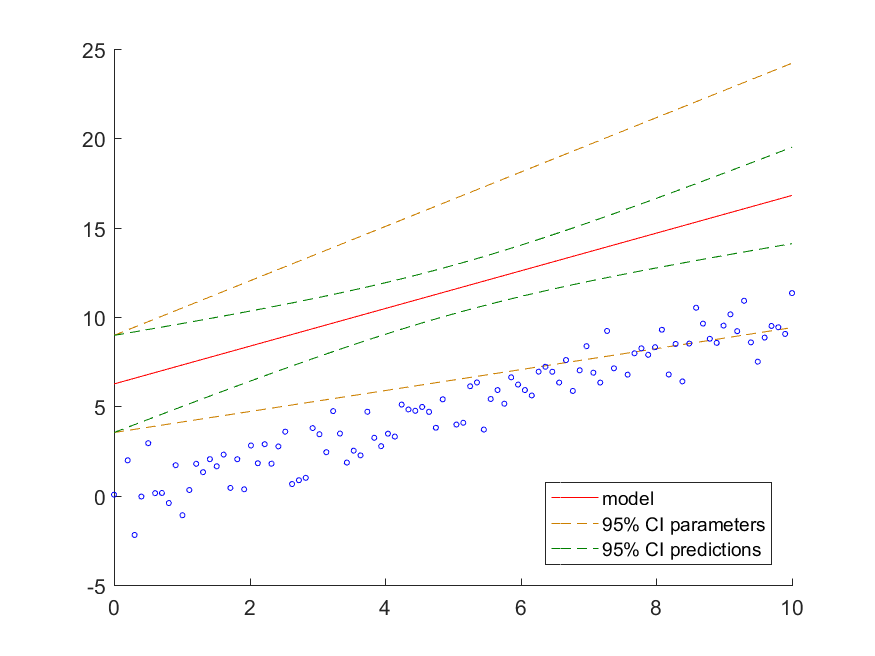
\includegraphics[width=0.6\textwidth]{../img/LInf_CI}
\caption{$L_\infty$ confidence intervals}
\label{fig:lInfCI}
\end{figure}

The histogram displayed in figure \ref{fig:lInfHist} confirms this. The residuals are completely different to to those of the true model, and the standard deviation of the noise wildly differs from that of the true model. In fact, it is nearly seven times greater (see Table 1).The size of the residuals makes the model considerably uncertain. Indeed, figure \ref{fig:lInfCI} shows the extremely wide confidence intervals of both the parameters and the predictions.

\newpage
\subsection{Huber Estimation}

So far we have studied models that are fed residuals directly. The Huber method, in contrast, is fed a residual function ($\varrho(t)$) that when treating the residuals shifts between two functions depending on the size of the residual. The discriminant variable $\tau$ is specified by the user, and its value should resemble the standard deviation of the data's noise. In our case, the data's noise standard deviation is 1.0293, and so we set $\tau = 1.0293$. We define the Huber function as follows:
\begin{equation}
\rho (t) = \begin{cases} \frac{1}{2} t^2, &  \vert t \vert \leq \tau \\ 
\tau \vert t \vert -\frac{1}{2} \tau^2, & \vert t \vert > \tau \end{cases}
\label{eq:Huber}
\end{equation}

\begin{figure}[htb]
\centering
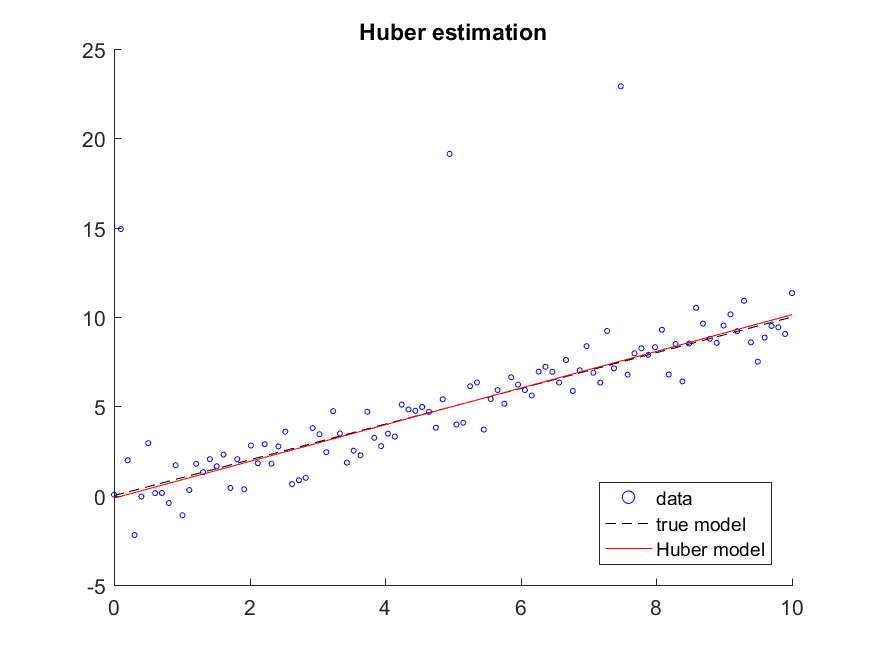
\includegraphics[width=0.6\textwidth]{../img/Huber}
\caption{Huber estimation}
\label{fig:HuberEstimation}
\end{figure} 

We can write the minimization problem  as:

\begin{equation}
\min\limits_{x \in \mathbb{R}^n} \phi = \sum_{i = 1}^m \rho ([A x - b]_i)
\label{eq:Huber2}
\end{equation}

To find a solution, we have to provide three new vectors $y$, $z$ and $w$ to our set of parameters. Equation \ref{eq:Huber2} takes then the form:


\begin{equation}
\min\limits_{x, y, z, w} \phi = \frac{1}{2} \mathbf{w}' \mathbf{w} + \tau [\mathbf{1}] (\mathbf{b} + \mathbf{z})
\label{eq:Huber3}
\end{equation}
\[
\mathbf{w} - \mathbf{A x} + \mathbf{b} - \mathbf{b} + \mathbf{z} = 0
\]
\[
\mathbf{b} \geq 0 \qquad \mathbf{z} \geq  0
\]

Which can be transformed into a quadratic problem:

\begin{equation}
\frac{1}{2} \mathbf{x' H x} + \mathbf{g' x} + \mathbf{\gamma} \qquad \mathbf{Ax} = \mathbf{b} \qquad l \leq x \leq u
\label{eq:Huber4}
\end{equation}

Where:

\[
\mathbf{H} =
\begin{bmatrix}
\mathbf{0} & \mathbf{0} & \mathbf{0} & \mathbf{0}\\
\mathbf{0} & \mathbf{0} & \mathbf{0} & \mathbf{0} \\
\mathbf{0} & \mathbf{0} & \mathbf{0} & \mathbf{0} \\
\mathbf{0} & \mathbf{0} & \mathbf{0} & \mathbf{I}
\end{bmatrix}
\qquad
\mathbf{g} = \tau
\begin{bmatrix}
\mathbf{0}\\
\mathbf{1}\\
\mathbf{1}\\
\mathbf{0}
\end{bmatrix}
\]

\[
\mathbf{A} = \begin{bmatrix}
-\mathbf{A} & -\mathbf{I} & \mathbf{I} & \mathbf{I}
\end{bmatrix} 
\qquad
\mathbf{b} = -\mathbf{b} 
\]

\[
\begin{bmatrix}
-\mathbf{\infty} & \mathbf{0} & \mathbf{0} & -\mathbf{\infty}
\end{bmatrix}'
\leq \mathbf{x} \leq 
\begin{bmatrix}
\mathbf{\infty} & \mathbf{\infty} & \mathbf{\infty} & \mathbf{\infty}
\end{bmatrix}'
\]


The vectors $\mathbf{b}$, $\mathbf{b}$ and $\mathbf{z}$ are all length $m$ (number of data points), thus, $\mathbf{0}$ are square matrices of zeros whose dimensions correspond to the length of the vectors they multiply, and $I$ is the identity matrix of dimension $m \times m$. 

\begin{figure}[htb]
\centering
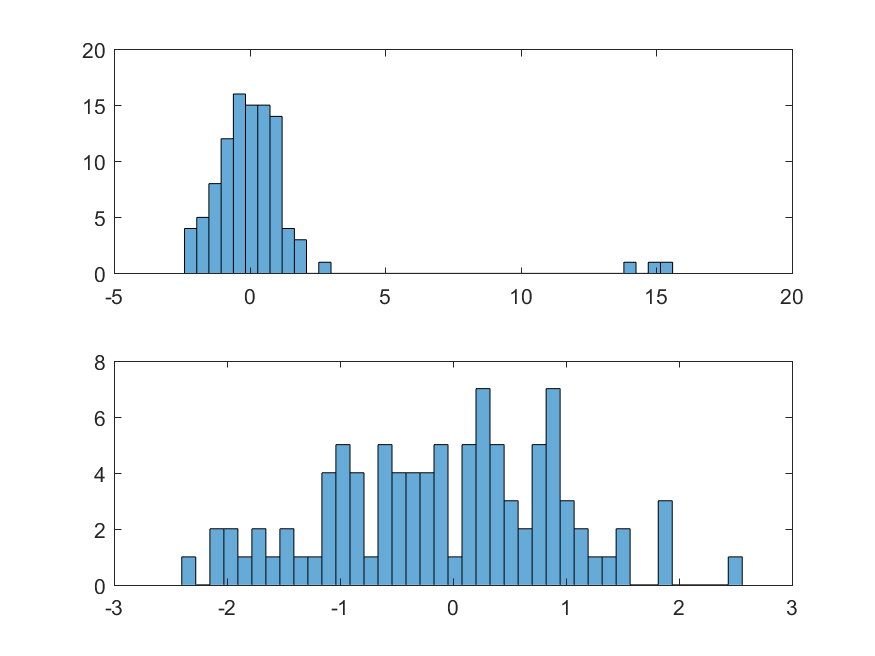
\includegraphics[width=0.6\textwidth]{../img/Huber_hist}
\caption{Huber histogram of the errors}
\label{fig:HuberHist}
\end{figure} 

Finally, we input these matrices to the linprog \matlab function to obtain our parameter estimates. We observe in figure \ref{fig:HuberEstimation} that the model  closely resembles the true model, and therefore is not sensitive to the three large positive outliers. From equation \ref{eq:Huber2}, we can see that the Huber estimator obtains robustness by alternating between the $L_2$ estimator and a hybrid of the $L_1$.



Since the estimated parameters are very close to the true parameter values, the histogram plot of the residuals in figure \ref{fig:HuberHist} shows again characteristics of a normal distribution.



\begin{figure}[htb]
\centering
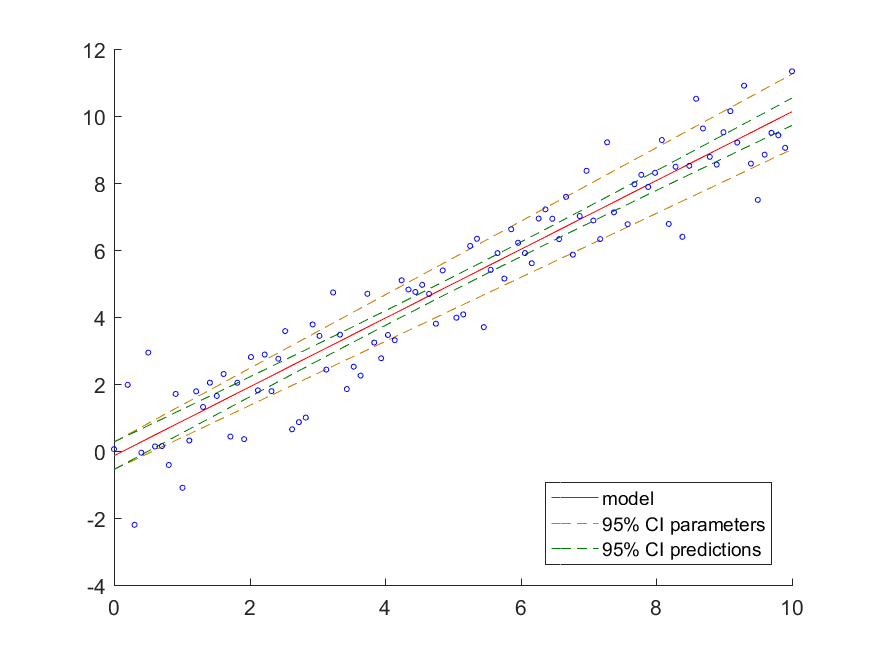
\includegraphics[width=0.6\textwidth]{../img/Huber_CI}
\caption{Huber confidence intervals}
\label{fig:HuberCI}
\end{figure} 


Figure \ref{fig:HuberCI} tells us that on aggregate the expected value of new observations would lie within that interval 95\% of the time.  The brown dashed lines, on the other hand, explain how much our model could vary if we used a different data sample from the same distribution.


\subsection{Method Comparison}

As mentioned in the introduction, a robust regression method could be described as one which incorporates potential outliers without being too sensitive to them. To that effect, we can test the quality of the methods studied in this report and assess their robustness. Table \ref{tab:table2} lists the parameter estimates and the uncertainty of those estimates for each method.  

Evidently, the best performer is $L_1$ followed closely by the Huber model in regards to parameter estimation. The $L_1$ model estimates the $\alpha$ and $\beta$ parameters more closely than all other methods while the uncertainty of the estimates (std. dev.) is relatively similar across all methods except for the $L_\infty$ model, which clearly is the underperformer of the group. The $L_2$ or LSQ method is sensitive to outliers as discussed in section 1.2. 

\begin{table}[htb]
\centering
\begin{tabular}{l|cccc} \hline \hline 
\multicolumn{5}{c}{Standard Deviation of Noise for Different Models} \\ \hline \hline
True Model & $L_2$ & $L_1$ & $L_\infty$ & Huber \\ \hline 
1.0293 & 1.1228 & 1.0339 & 6.9085 & 1.025  \\ 
\hline 
\end{tabular}C
\caption{}
\label{tab:table1}
\end{table}



Ultimately, the reason behind this is that the loss function of the LSQ ($0.5r^{2}$) model grows faster (than that of Huber and $L_1$) as the magnitude of the residuals increase (see Figure \ref{fig:ResMag}). Since the $L_2$ minimizes the sum of the squared residuals, outliers greater than one will have a bigger influence ($e^2$  -vs- $e$) than in the $L_1$ model. Consequently, the $L_2$ is much more vulnerable to outliers as the model has to adjust to minimize these larger values. Under this light, it is not surprising to see that the $L_\infty$ performs so poorly: since it minimizes the maximum value, it is extremely sensitive to outliers.  

 \begin{figure}[htb]
\centering
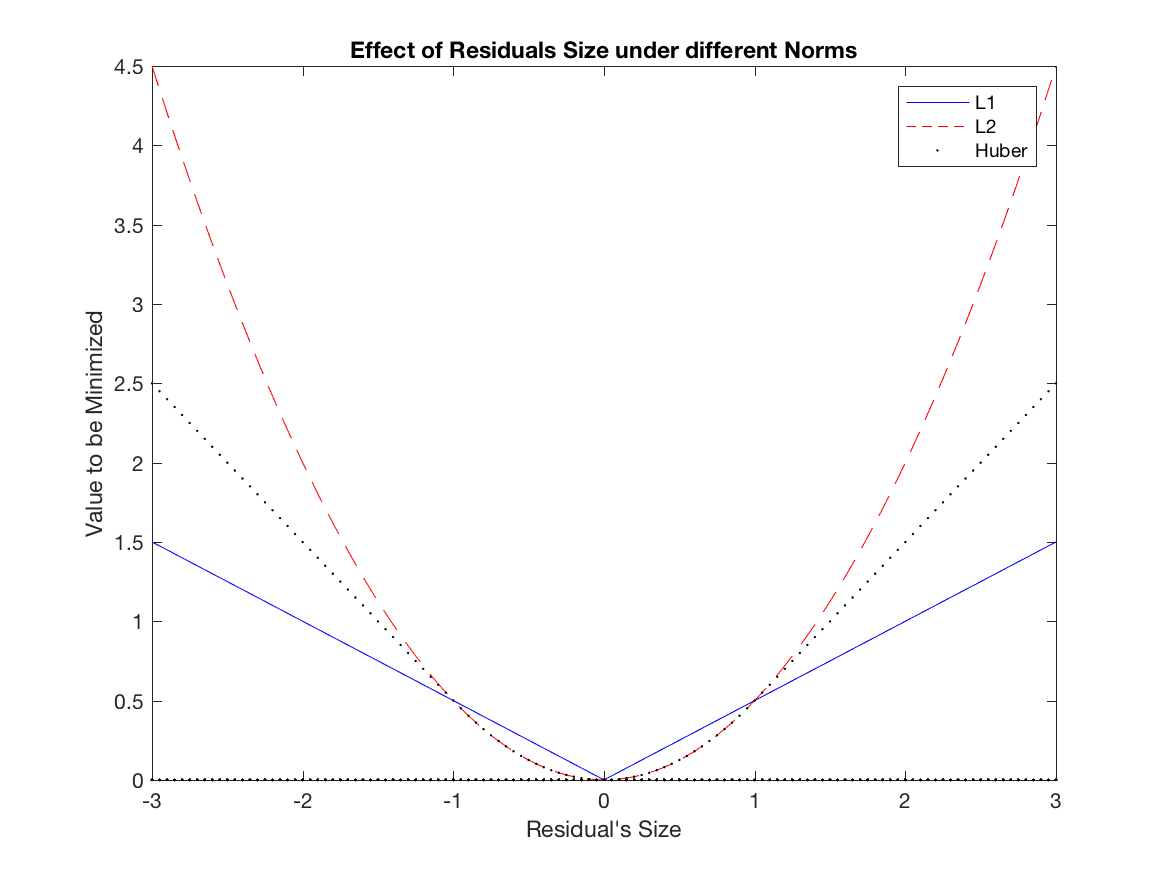
\includegraphics[width=0.85\textwidth]{../img/ResMag}
\caption{The effect of the residuals' magnitude on the minimization task is shown above for each of the estimators. Above, $tau$ is set equal to $1.023$ which mirrors the standard deviation of data's noise.}
\label{fig:ResMag}
\end{figure} 

%This was the paragraph marked for deletion
For very small residual values, both the Huber and the $L_2$ loss functions grow slower than the $L_1$ (see Figure \ref{fig:ResMag}). However, outside this small range as the residuals' magnitude increases, the $L_2$ loss function grows faster (quadratically). In contrast, the loss function of $L_1$ grows linearly and consequently can better handle outliers. 

In terms of computational efficiency, since $L_2$ is differentiable and smooth, a unique analytical solution can be found. The $L_1$ holds no such advantage and is therefore more computationally expensive (see Table \ref{tab:tableCPU}).  

\begin{table}[htb]
\centering
\begin{tabular}{cccc} \hline \hline 
\multicolumn{4}{c}{Computational Efficiency (in seconds)} \\ \hline \hline
$L_2$ & $L_1$ & $L_\infty$ & Huber \\ \hline 
0.0026 & 0.0621 & 0.0599 & 0.0141  \\ 
\hline 
\end{tabular}
\caption{The elapsed time is computed as an average of 100 iterations.}
\label{tab:tableCPU}
\end{table}

The advantage of the Huber formulation is that it incorporates the smoothness of the LSQ with the robustness of $L_1$. By combining these two features, it is able to handle outliers (like the $L_1$) while also finding a unique, stable solution with computational efficiency (like the $L_2$). Furthermore, another benefit of Huber is that the user can specify what exactly constitutes a large or small residual (to target outliers)  by manipulating the value of $tau$. Therefore, the user's knowledge of the data and the problem at hand can be leveraged by assigning an appropriate $\tau$ value, which should reflect the standard deviation of the data's noise. 

In conclusion, the $L_1$ provides robustness but it's not computationally efficient, relatively speaking, while the $L_2$ has the reverse trade-off.  Therefore, the $L_1$ estimator is better suited for applications where  large outliers are likely and can be justifiably ignored, such as seismic-inverse problems. For applications where the information provided by outliers is important the $L_2$ estimator is more apt. Finally, the Huber method captures the advantages of both worlds.


\vspace*{\fill} 
\begin{table}[htb]
\centering
\begin{tabular}{l|cccc|cc} \hline \hline 
\multicolumn{7}{c}{$L_2$ Model} \\ \hline \hline
Parameter & Estimate & Std. Dev. & Lower Bound & Upper Bound & \multicolumn{2}{c}{Covariance}  \\& & & & & $\alpha$ & $\beta$ \\ \hline 
$\alpha$ & 0.9943 & 0.0392 & 0.9178 & 1.0707 & 0.0015 & \\ 
$\beta$ & 0.3967 & 0.2277 & -0.0456 & 0.8390 & -0.0077 & 0.0518 \\ 
\hline \hline 
\multicolumn{7}{c}{$L_1$ Model} \\ \hline \hline
Parameter & Estimate & Std. Dev. & Lower bound & Upper bound & \multicolumn{2}{c}{Covariance}  \\& & & & & $\alpha$ & $\beta$ \\ \hline 
$\alpha$ & 0.9971 & 0.0361 & 0.9254 & 1.0688 & 0.0013 & \\ 
$\beta$ & 0.0530 & 0.2096 & -0.3632 & 0.4692 & -0.0066 & 0.0439 \\ 
\hline \hline 
\multicolumn{7}{c}{$L_\infty$ Model} \\ \hline \hline
Parameter & Estimate & Std. Dev. & Lower bound & Upper bound & \multicolumn{2}{c}{Covariance}  \\& & & & & $\alpha$ & $\beta$ \\ \hline 
$\alpha$ & 1.0556 & 0.2335 & 0.5921 & 1.5191 & 0.0545 & \\ 
$\beta$ & 6.2502 & 1.3517 & 3.5677 & 8.9327 & -0.2727 & 1.8272 \\ 
\hline \hline 
\multicolumn{7}{c}{Huber Model} \\ \hline \hline
Parameter & Estimate & Std. Dev. & Lower bound & Upper bound & \multicolumn{2}{c}{Covariance}  \\& & & & & $\alpha$ & $\beta$ \\ \hline 
$\alpha$ & 1.0278 & 0.0358 & 0.9567 & 1.0988 & 0.0013 \\ 
$\beta$ & -0.1256 & 0.2078 & -0.5382 & 0.2870 & -0.0064 & 0.0432 \\ 
\hline \hline
\end{tabular} 
\caption{The bounds on the parameter's estimates are computed as $95\%$ confidence intervals. }
\label{tab:table2}
\end{table}
\vspace*{\fill} 
